\subsection{Ablauf}

Im Sequenzdiagramm sieht man den Ablauf der ganzen Applikation, sowohl Desktop Seite wie auch Smartphone Seite. Da die Aufgabe vom Gerät völlig autonom verrichtet werden muss wird nach dem Start der Android-App das Smartphone nicht mehr bedient werden und alle Interaktionen werden von der Desktop-App gesteuert. 
Wie aus dem Sequenzdiagramm zu entnehmen ist wird auf der Android-App als erstes ein Foto geschossen mithilfe dessen dann die Korberkennung erfolgt. Wurde das Startsignal von der Desktopp-App mit übergeben richtet sich das Gerät dann aus und schiesst die Bälle ab. Danach wird das Endsignal an die Desktopp-App übergeben.
Falls das Startsignal nicht übergeben wurde wird die Korberkennung dennoch ausgeführt allerdings schiesst das Gerät die Bälle nicht ab, dies wird für das Testen benötigt um zu überprüfen ob die Korberkennung wie gewünscht funktioniert.


\begin{figure}[h!]
	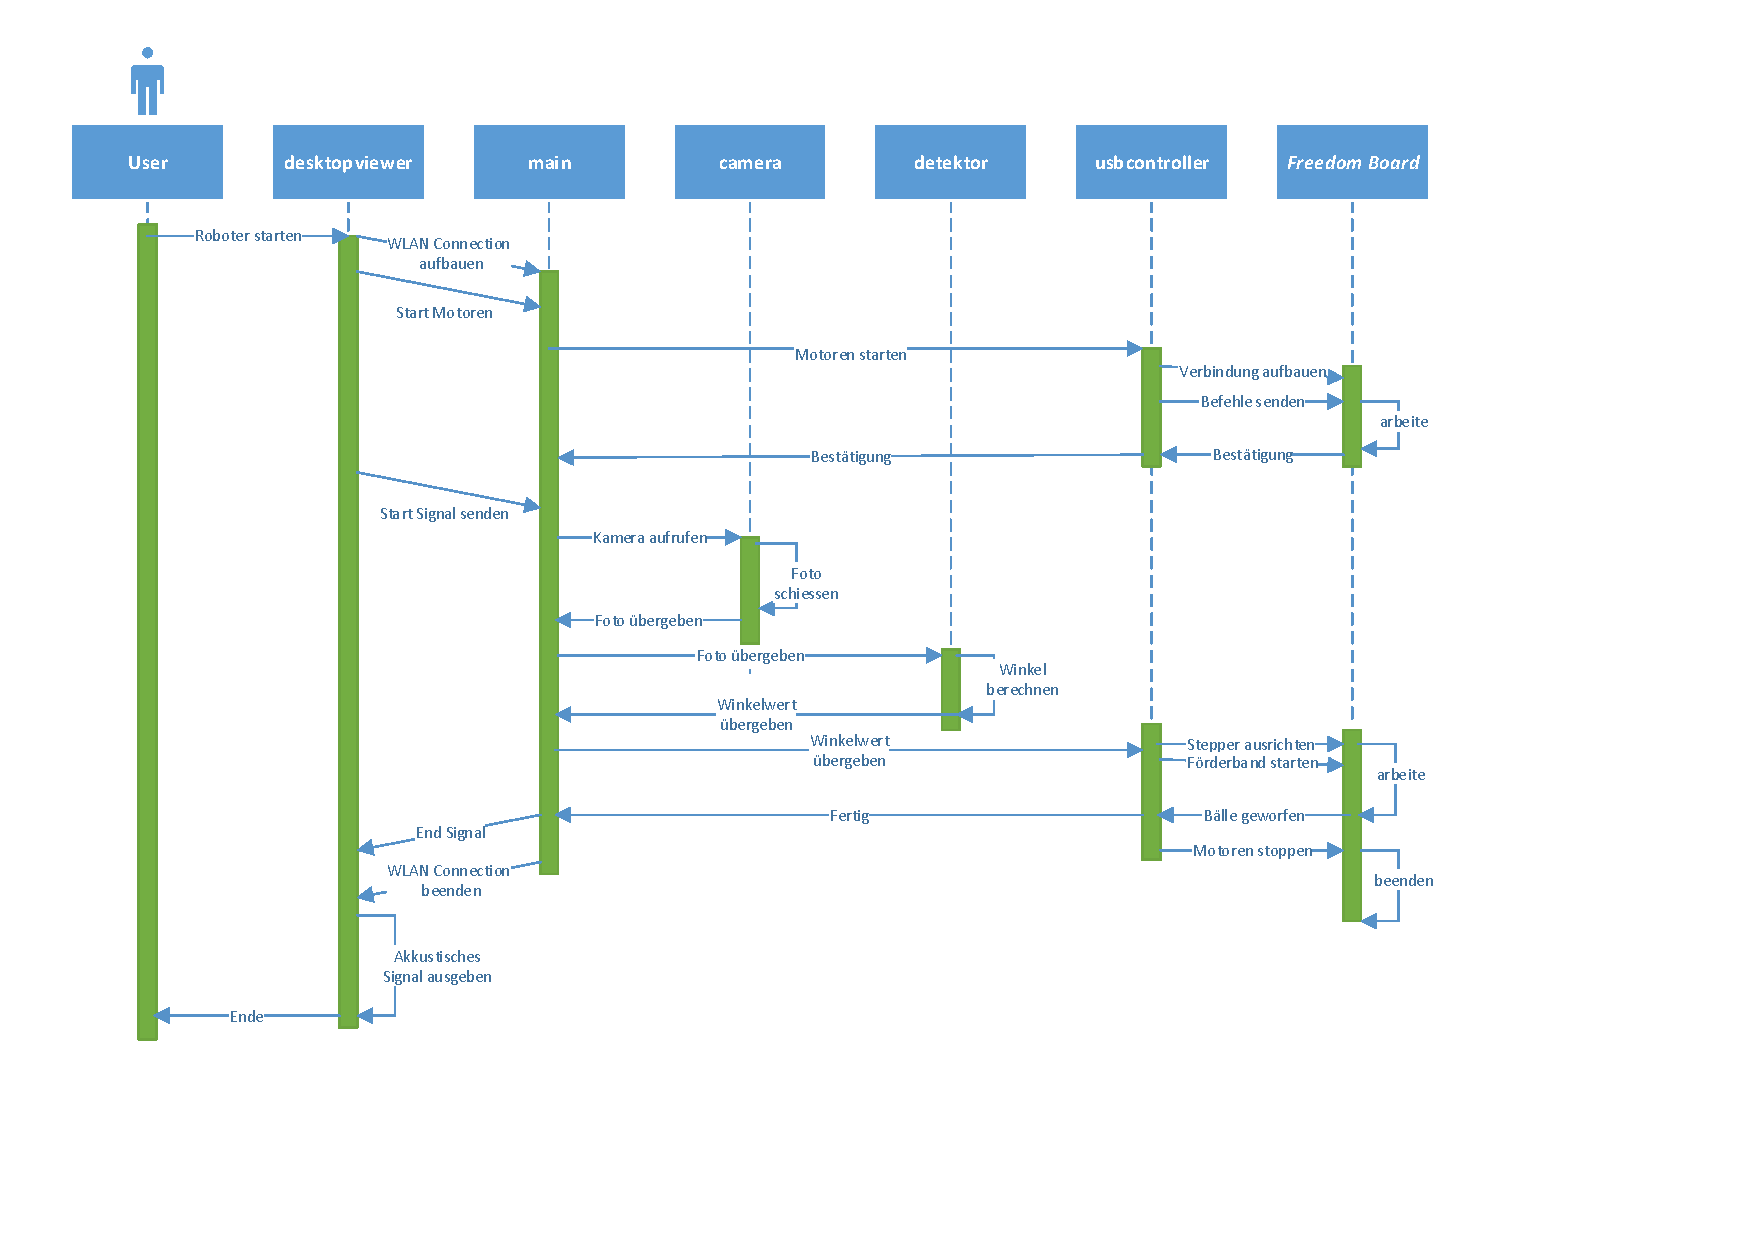
\includegraphics[width=\textwidth]	{Enddokumentation/Bilder/Sequenzdiagramm_PREN2_v1.pdf}
	\centering
	\caption{Sequenzdiagramm Programmablauf}
	\label{abb:SequenzdiagrammSoftware}
\end{figure}


            
